\noindent El diseño del dedo exoesqueleto con 6 GDL se muestra en la Figura \ref{fig:3DModel} en su posición inicial de
"CASA" y está constituido por una cadena cinemática de 7 eslabones, que están todos conectados entre sí por articulaciones
revolutas. El software que se utilizó para generar el diseño en 3D, fue solidworks porque tiene varias herramientas que
ayudaron en el desarrollo matemático, así como su versatilidad para enlazarse con matlab, software con el que se
programaron los cálculos.  
\begin{figure}[H]
    \centering
    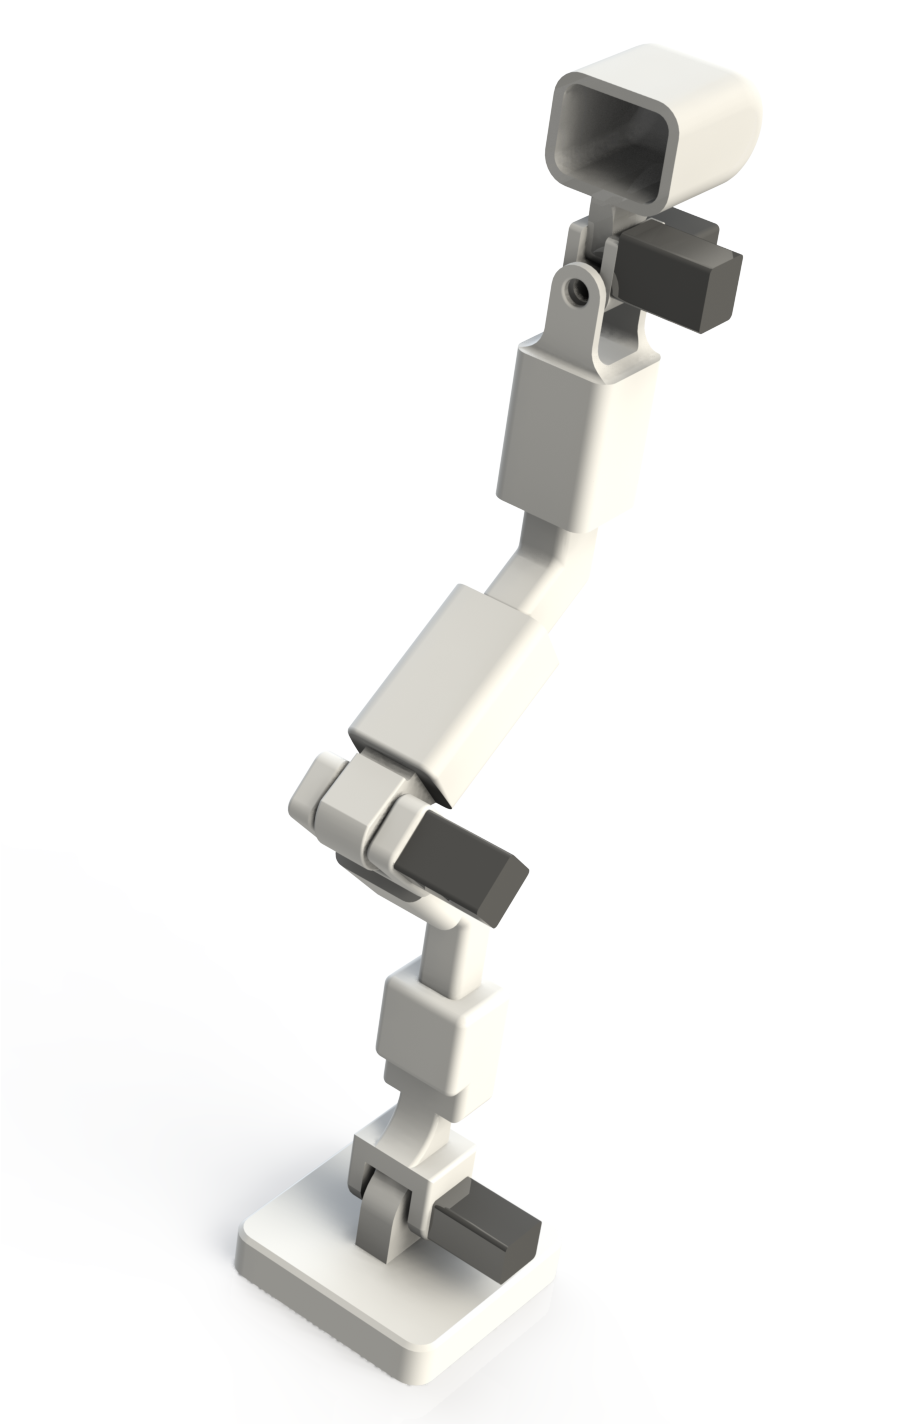
\includegraphics[scale=0.3]{Dedo Vist Isometrica.png} 
    \caption{Diseño 3D}
    \label{fig:3DModel}
\end{figure}

\subsection{Diseño del exoesqueleto}
\noindent La disposición de las articulaciones que se muestran en la Figura \ref{fig:EsqArtOri}, fueron las planteadas
originalmente en el manual de robótica, proporcionado por el Dr. Ernesto Olguín.

\begin{figure}[H]
    \centering
    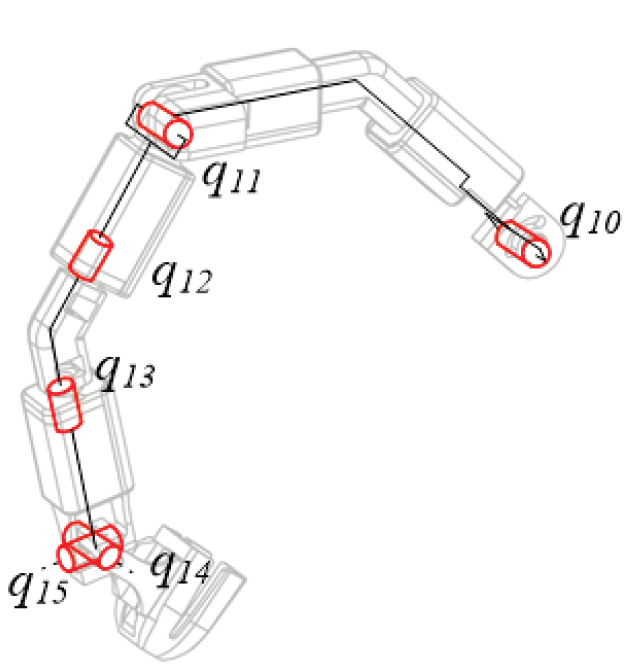
\includegraphics[scale=0.5]{EsquemaArticulaciones.png} 
    \caption{Esquema de las Articulaciones Original}
    \label{fig:EsqArtOri}
\end{figure}
\noindent Sin embargo por cuestiones de practicidad el equipo propuso una modificación y se agregó un eslabón más, de
esta manera se evita que la articulación revoluta  $q_5$ y  $q_6$ estuvieran fusionadas, como se visualiza en la 
Figura \ref{fig:EsqArtOri}. El dibujo posicionado con una perspectiva lateral derecha, que se visualiza en la Figura 
\ref{fig:ExoPara} proporciona una imagen con dimensiones parametrizadas, mismas que se plasman en la siguiente tabla: 

\begin{table}[!ht] %[H]
    \centering
    \begin{center}
        \begin{tabular}{ccc}
            Parámetros & [m] & [rad] \\
            \hline \hline 
            L1 & 0.03235525 & \\ 
            L2 & 0.10513390 & \\
            L3 & 0.02462267 & \\
            L4 & 0.02228474 & \\
            L5 & 0.04334075 & \\
            L6 & 0.00600000 & \\
            L7 & 0.01999013 & \\
            L8 & 0.02565247 & \\
            L9 & 0.01273194 & \\
            L10 & 0.03641522 & \\
            $\alpha$ &  & 59.26721315°\\
        \end{tabular}
    \end{center}
\end{table}
Así mismo, en la Figura \ref{fig:ExoPara} se aprecia la asignación de referenciales $q_1$, $q_2$, $q_3$, $q_4$, $q_5$
y $q_6$. Los marcos inerciales propuestos a cada GDL se colocaron utilizando la convención GRyMA, manteniendo la
dirección positiva de la mano derecha.
    
También se asignaron materiales, proponiendo para los eslabones un polímero termoplástico de nombre "acrilonitrilo
butadieno estireno" también conocido como filamento ABS, utilizado por impresoras 3D, pensando que en un futuro próximo
podamos imprimir el modelo y así experimentar con el en un entorno real; en el caso del dedal, se seleccionó un polímero artificial que pertenece al grupo de las poliamidas, llamado comunmente "Nylon", pues creemos que para cuidar la comodidad del usuario, al ingresar su dedo, el material no debe ser tan rígido y el nylon permite un equilibrio entre la suavidad y al mismo tiempo que no sea deformable.
Finalmente los motores propuestos son de micro Metal LP con reductora de 50:1, de corriente continua, con dimensiones
de 24 x 10 x 12 mm y 10 gramos de peso \\ 
\begin{figure} [h!]
            \centering
            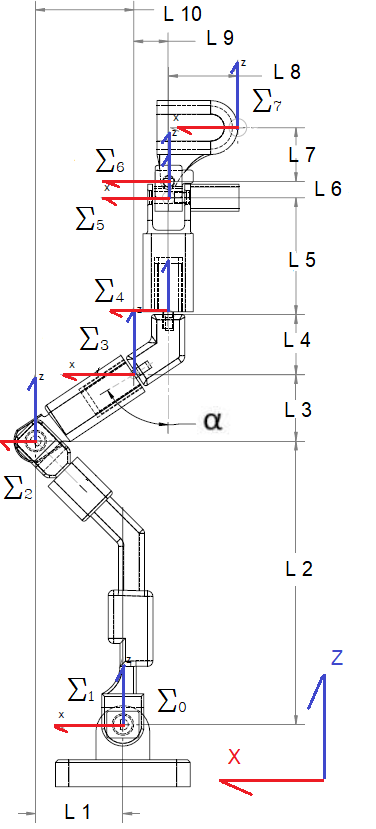
\includegraphics[scale=0.7]{ExoParametrizado.png}
        \caption{Esquema de las Articulaciones Utilizado}
        \label{fig:ExoPara}
\end{figure}
\noindent  \\
Conocer la cantidad de grados de libertar que tiene el exoesqueleto, nos servirá para identificar la versatilidad del
movimiento que se podrá ejercer. Existen 3 clasificaciones [2] :
\begin{itemize}
    \item Menos de 6 GDL. Tienen menos GDL que el movimiento que puede tener en el espacio. Es decir, si el robot está
    diseñado para moverse en un espacio tridimensional (con 3 parámetros de traslación y 3 de rotación) y tiene menos
    de 6 GDL, presentará  limitaciones en la manera en que se mueve. 
    \item Exactamente 6 GDL. Para aquellos manipuladores robóticos que tienen exactamente 6 GDL, pueden mover su efector
    final de manera independiente en cada uno de los seis parámetros que conforman el espacio de trabajo tridimensional.
    \item Más de 6 GDL. Si un robot tiene más actuadores que los parámetros del espacio en el que se puede mover,
    implica que está sobre actuado y por lo tanto redundante.
\end{itemize}